%-*-latex-*-
If you know the game Reversi, you will recognize that this program is part of
the logic in a $1$--dimensional version of Reversi. Before we talk about the
program you need to write, let me first talk about Reversi.

In the game of Reversi, if you put your piece on the board at an empty spot,
you capture all the enemy pieces that form a straight line which are between
the piece you put down and another one of your pieces. When a piece is
captured, it becomes one of your pieces. Here's an example using a $5$--by--$5$
Reversi board (the actual Reversi is larger). I use \verb!@! for a black piece
and \verb!O! for a white piece. Here's the board:

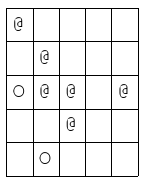
\includegraphics[scale=0.5]{pic1.png}

Now you put down your \verb!O!:

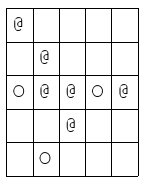
\includegraphics[scale=0.5]{pic2.png}

The \verb!@! pieces which are captured becomes you pieces. For instance, the
two \verb!@! pieces shown are captured:

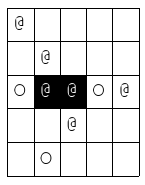
\includegraphics[scale=0.5]{pic3.png}

So is this one:

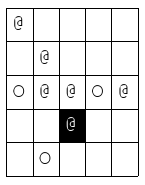
\includegraphics[scale=0.5]{pic4.png}

The captured pieces become yours so the board becomes:

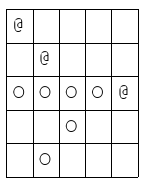
\includegraphics[scale=0.5]{pic5.png}

Note that there must not be a gap between the pieces for the enemy pieces
between two of your pieces to get captured. For instance, if the board looks
like this:

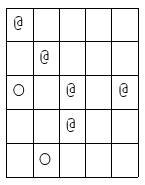
\includegraphics[scale=0.5]{pic6.png}

Then putting your piece at the same spot will result in this:

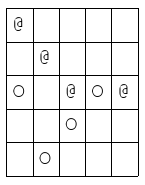
\includegraphics[scale=0.5]{pic7.png}

The \verb!O! piece to the left of the piece you put down does not capture the
\verb!@! on the left because there is a gap in-between.
(Talk to me if you do not understand the rule of the game.)

For this question, you will write a program to perform only one step in the
game and furthermore, this is a $1$--dimensional version with $15$ spots:

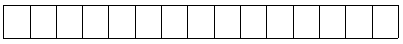
\includegraphics[scale=0.5]{pic8.png}

We will use an array of $15$ integers to represent our $1$--dimensional Reversi
board. Furthermore, I will use zero ($0$) in the array to represent a blank
space, $1$ to represent a white piece and $2$ to represent a black piece.

You are given the following skeleton code. It declares an array of $15$
integers and then prompts the user for $15$ integers to be placed into the
array. The array models our $1$--dimensional Reversi board.

The user (i.e., you) then enters an integer value into variable \verb!s!. This
is the index of the array where you want to put your piece which is $1$ (i.e.,
a white piece).

You need to write code at the indicated place in the code provided below to model
putting your piece on the board and capturing pieces if necessary.

The program ends by printing all the integers in the array.

Read the test cases carefully before programming.

\begin{Verbatim}[frame=single]
// Name:
// File:

#include <iostream>

int main()
{
    int SIZE = 15;
    int a[SIZE];

    // YOUR CODE HERE

    return 0;
}
\end{Verbatim}


\resett
\nextt
\begin{console}[frame=single, commandchars=\\\{\}]
\userinput{0 0 0 0 1 0 0 0 0 0 0 0 0 0 0}
board: 000010000000000
index to put a 1: \userinput{4}
board: 000010000000000
\end{console}
As you can see, at index $4$, there is already a $1$ (i.e., it's not a blank
spot since it's not a $0$.) This is therefore not a valid move.

\nextt
\begin{console}[frame=single, commandchars=\\\{\}]
\userinput{0 0 0 0 2 0 0 0 0 0 0 0 0 0 0}
board: 000020000000000
index to put a 1: \userinput{4}
board: 000020000000000
\end{console}
This is similar to \textsc{Test 1}; it's not a valid move.

\nextt
\begin{console}[frame=single, commandchars=\\\{\}]
\userinput{0 0 0 0 0 0 0 0 0 0 0 0 0 0 0}
board: 000000000000000
index to put a 1: \userinput{4}
board: 000010000000000
\end{console}
In this case, the spot at index $4$ is not taken. Therefore, your piece (i.e.,
$1$) is placed at index $4$. However, you did not capture any enemy piece.

\nextt
\begin{console}[frame=single, commandchars=\\\{\}]
\userinput{0 0 0 0 0 2 1 0 0 0 0 0 0 0 0}
board: 000002100000000
index to put a 1: \userinput{4}
board: 000011100000000
\end{console}
In this case, you captured an enemy piece to the right (i.e., you captured a
$2$, which becomes your piece.)

\nextt
\begin{console}[frame=single, commandchars=\\\{\}]
\userinput{0 0 0 0 0 0 0 0 2 2 2 1 0 0 0}
board: 000000002221000
index to put a 1: \userinput{7}
board: 000000011111000
\end{console}
In this case, you captured three enemy pieces to the right.

\nextt
\begin{console}[frame=single, commandchars=\\\{\}]
\userinput{0 0 0 0 0 0 0 2 2 2 0 1 0 0 0}
board: 000000022201000
index to put a 1: \userinput{6}
board: 000000122201000
\end{console}
In this case, you did not capture any pieces since there is a $0$ (i.e., empty
space) between the $2$s between the $1$ you put down and the other $1$ already
on the board.

\nextt
\begin{console}[frame=single, commandchars=\\\{\}]
\userinput{0 0 0 0 0 0 0 0 2 2 2 1 0 0 0}
board: 000000002221000
index to put a 1: \userinput{6}
board: 000000102221000
\end{console}
This is similar to \textsc{Test 6}.

\nextt
\begin{console}[frame=single, commandchars=\\\{\}]
\userinput{0 0 0 0 0 1 2 2 2 2 0 0 0 0 0}
board: 000001222200000
index to put a 1: \userinput{10}
board: 000001111110000
\end{console}
In this case you captured four pieces to the left of the piece you put down.

\nextt
\begin{console}[frame=single, commandchars=\\\{\}]
\userinput{0 0 0 1 0 2 2 2 2 0 0 0 0 0 0}
board: 000102222000000
index to put a 1: \userinput{9}
board: 000102222100000
\end{console}
In this case you did not capture any piece.

\nextt
\begin{console}[frame=single, commandchars=\\\{\}]
\userinput{0 0 0 1 2 2 2 2 2 0 2 2 2 1 0}
board: 000122222022210
index to put a 1: \userinput{9}
board: 000111111111110
\end{console}
In this case you captured $5$ pieces to the left and three pieces to the right
of the piece you put down.

\nextt
\begin{console}[frame=single, commandchars=\\\{\}]
\userinput{0 0 0 1 2 2 2 2 2 0 2 2 2 2 2}
board: 000122222022222
index to put a 1: \userinput{9}
board: 000111111122222
\end{console}
In this case you captured 5 pieces to the left.

\nextt
\begin{console}[frame=single, commandchars=\\\{\}]
\userinput{0 0 0 0 0 0 0 0 0 0 0 0 2 2 2}
board: 000000000000222
index to put a 1: \userinput{11}
board: 000000000001222
\end{console}
In this case there are no captures because of obvious reasons.
Make sure that this case works in the other direction as well.

\textsc{Advice}:
Focus on capturing to the right first. Once you're done with that (and
it's completely tested!), making it work for capturing to the left should be
easy.
